\chapter{Postavy}

\begin{comment}
\begin{figure}[!h]
\begin{minipage}[t]{\minipageSize}\centering
  \includegraphics[width=\cardSize\linewidth]{}
 \caption[]{}
  \label{fig:bang}
\end{minipage}
\hfill
\begin{minipage}[t]{\minipageSize}\centering
  \includegraphics[width=\cardSize\linewidth]{}
  \caption[]{}
  \label{fig:vedle}
\end{minipage}
\hfill
\begin{minipage}[t]{\minipageSize}\centering
  \includegraphics[width=\cardSize\linewidth]{}
  \caption[]{}
  \label{fig:duel}
\end{minipage}
\hfill
\begin{minipage}[t]{\minipageSize}\centering
  \includegraphics[width=\cardSize\linewidth]{}
\caption[]{}
  \label{fig:panico}
\end{minipage}
\end{figure}
\end{comment}
\begin{figure}[!h]
\begin{minipage}[t]{\minipageSize}\centering
  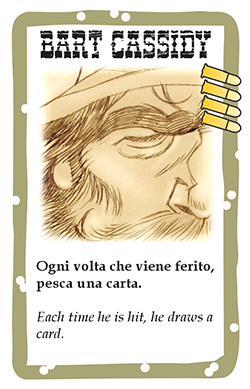
\includegraphics[width=\cardSize\linewidth]{postavy/01_bartcassidy.png}
 \caption[Bart Cassidy]{Kedykoľvek je stratí život a prežije, potiahne si kartu z balíka. V prípade dynamitu (ak prežije alebo sa zachráni pivom) ťahá 3 karty.}
  \label{fig:bang}
\end{minipage}
\hfill
\begin{minipage}[t]{\minipageSize}\centering
  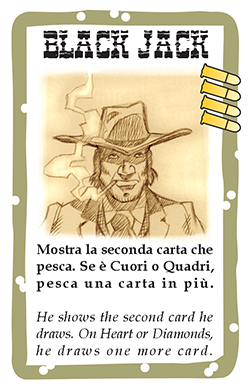
\includegraphics[width=\cardSize\linewidth]{postavy/01_blackjack.png}
  \caption[Black Jack]{Vo fáze 1 ukáže druhú kartu ktorú si potiahol. Ak je červená tak si potiahne ešte jednu kartu (neukazuje ju).}
  \label{fig:vedle}
\end{minipage}
\hfill
\begin{minipage}[t]{\minipageSize}\centering
  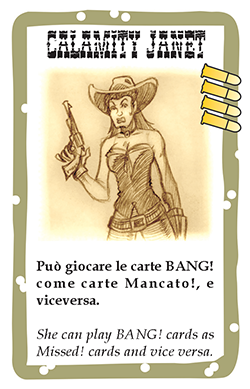
\includegraphics[width=\cardSize\linewidth]{postavy/01_calamityjanet.png}
  \caption[Calamity Janet]{Môže zahrať kartu Bang! ako kartu Vedle! a naopak. Karta Vedle! zahraná ako karta Bang! sa počíta do limitu Bang!.}
  \label{fig:duel}
\end{minipage}
\hfill
\begin{minipage}[t]{\minipageSize}\centering
  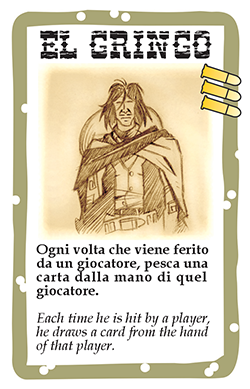
\includegraphics[width=\cardSize\linewidth]{postavy/01_elgringo.png}
\caption[El Gringo]{Kedykoľvek stratí život vďaka karte zahranej iným hráčom, vezme si jednu náhodnú kartu z ruky tohto hráča za každý takto stratený život. Ak útočiaci hráč už nemá žiadne karty na ruke, El Gringo si nič nevezme. Schopnosť neplatí pri Dynamite a pri Duele, ktorý vyvolal sám El Gringo.}
  \label{fig:panico}
\end{minipage}
\end{figure}
\begin{figure}[!h]
\begin{minipage}[t]{\minipageSize}\centering
  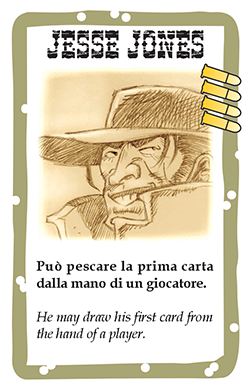
\includegraphics[width=\cardSize\linewidth]{postavy/01_jessejones.png}
 \caption[Jesse Jones]{Vo fáze 1 si môže prvú kartu potiahnúť z ruky niektorého hráča.}
  \label{fig:bang}
\end{minipage}
\hfill
\begin{minipage}[t]{\minipageSize}\centering
  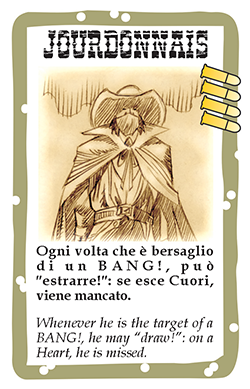
\includegraphics[width=\cardSize\linewidth]{postavy/01_jourdonnais.png}
  \caption[Jourdonnais]{Má pasívny Barel. Pri zásahu efektom Bang! môže ťahať vrchnú kartu balíčka; ak je srdcová, získa efekt Vedle!. Zároveň môže mať vyloženú aj kartu Barel. V takom prípade ťahá na každý efekt Bang! dvakrát.}
  \label{fig:vedle}
\end{minipage}
\hfill
\begin{minipage}[t]{\minipageSize}\centering
  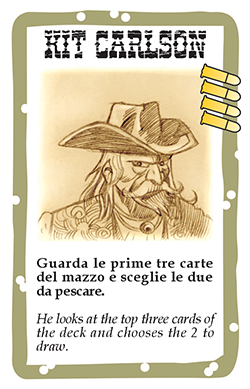
\includegraphics[width=\cardSize\linewidth]{postavy/01_kitcarlson.png}
  \caption[Kit Carlson]{Vo fáze 1 sa pozrie na 3 vrchné karty a potiahne 2 z nich. Tretiu zahodí.}
  \label{fig:duel}
\end{minipage}
\hfill
\begin{minipage}[t]{\minipageSize}\centering
  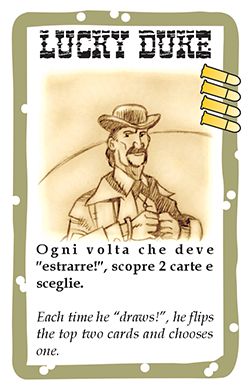
\includegraphics[width=\cardSize\linewidth]{postavy/01_luckyduke.png}
\caption[Lucky Duke]{Môže ťahať na efekt (napr. barrel a dynamit) dva krát. }
  \label{fig:panico}
\end{minipage}
\end{figure}

\begin{figure}[!h]
\begin{minipage}[t]{\minipageSize}\centering
  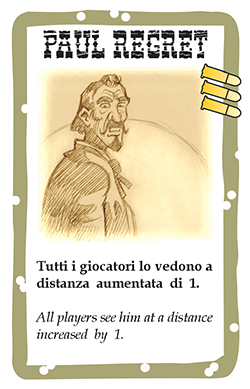
\includegraphics[width=\cardSize\linewidth]{postavy/01_paulregret.png}
 \caption[Paul Regret]{Vzdialenosť od všetkých hráčov je +1. Stackuje sa s Mustang, Skrýš etc.}
  \label{fig:bang}
\end{minipage}
\hfill
\begin{minipage}[t]{\minipageSize}\centering
  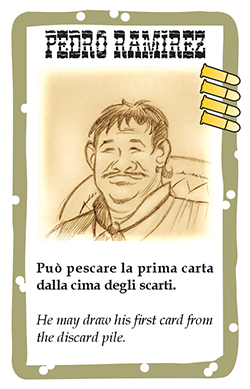
\includegraphics[width=\cardSize\linewidth]{postavy/01_pedroramirez.png}
  \caption[Pedro Ramiréz]{Vo fáze 1 si môže prvú kartu potiahnuť buď z vrchu odhadzovacej kopy, alebo z balíčka. Druhú kartu si potom vždy potiahne z balíčka. V situácii, keď sú v hre poslední dvaja hráči a Pedro dá svojho oponenta do Väzenia, môže sa podľa dohody hrať tak, že sa Väzenie točí dovtedy, kým sa z neho oponent nedostane.}
  \label{fig:vedle}
\end{minipage}
\hfill
\begin{minipage}[t]{\minipageSize}\centering
  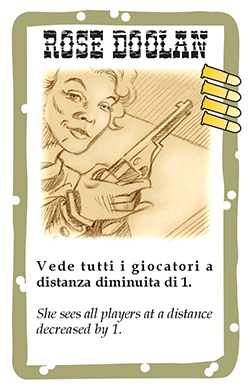
\includegraphics[width=\cardSize\linewidth]{postavy/01_rosedoolan.png}
  \caption[Rose Doolan]{Z jej perspektívy je vzdialenosť od všetkých hráčov -1. Platí aj na Paniku, Pepperbox etc.}
  \label{fig:duel}
\end{minipage}
\hfill
\begin{minipage}[t]{\minipageSize}\centering
  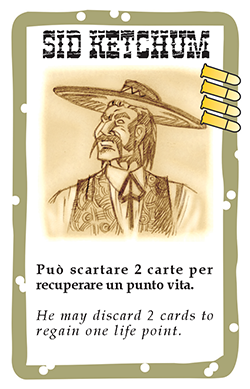
\includegraphics[width=\cardSize\linewidth]{postavy/01_sidketchum.png}
\caption[Sid Ketchum]{Za 2 vyhodené karty si môže doplniť jeden život (v rámci limitu). Túto schopnosť môže využiť mimo svoj ťah, aj na záchranu pred smrteľnou ranou ako pivo. Tak isto môže využiť svoju schopnosť keď sú dvaja hráči v hre.}
  \label{fig:panico}
\end{minipage}
\end{figure}

\begin{figure}[!h]
\begin{minipage}[t]{\minipageSize}\centering
  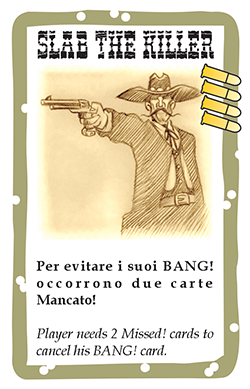
\includegraphics[width=\cardSize\linewidth]{postavy/01_slab.png}
 \caption[Slab The Killer]{Proti vašej karte Bang! potrebuje cieľ 2 efekty Vedle!; to neplatí na Derringer, Kulomet, Dvojitú ránu a podobné efekty. Keďže stále ide o jeden zosilnený efekt Bang!, na Barel sa ťahá iba raz. Ak je vytiahnutá karta srdcová, hráč musí zahrať ešte jeden efekt Vedle!; to platí aj pre Jourdonnaisa. \cite{Bang-Slab} Pri Opětovnej palbe stačí proti Slabovi iba 1 efekt Vedle!. Pri vyhýbaní sa Úhybom alebo Bibliou môže hráč zahrať aj práve potiahnutú kartu s efektom Vedle!.}
  \label{fig:bang}
\end{minipage}
\hfill
\begin{minipage}[t]{\minipageSize}\centering
  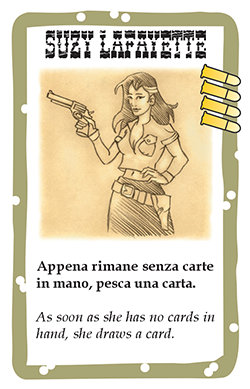
\includegraphics[width=\cardSize\linewidth]{postavy/01_suzylafayette.png}
  \caption[Suzy Lafayette]{Kedykoľvek nemá na ruke žiadnu kartu, potiahne si 1 kartu. Pri Dueli si kartu potiahne až po jeho skončení, nie počas neho. Ak po nej vystrelí Slab The Killer a Suzy má na ruke iba jednu kartu s efektom Vedle!, môže ju zahrať a následne si potiahnuť ďalšiu kartu. Ak má aj táto karta efekt Vedle!, môže ju zahrať a zrušiť ňou Bang! od Slaba.}
  \label{fig:vedle}
\end{minipage}
\hfill
\begin{minipage}[t]{\minipageSize}\centering
  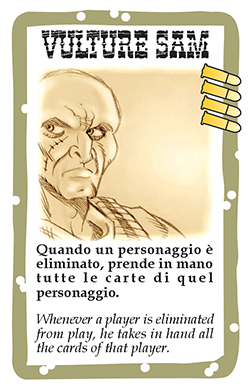
\includegraphics[width=\cardSize\linewidth]{postavy/01_vulturesam.png}
  \caption[Vulture Sam]{Kedykoľvek je hráč vyradený z hry, vezme si do ruky všetky karty tohto hráča na ruke a na stole (dynamit v prípade že nevybuchol, väzenie etc.). V prípade že je Vulture šerif a zabije Vice, najprv zoberie všetky jeho karty a potom ich odhodí.}
  \label{fig:duel}
\end{minipage}
\hfill
\begin{minipage}[t]{\minipageSize}\centering
  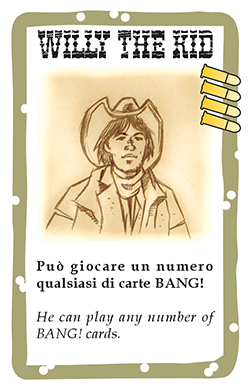
\includegraphics[width=\cardSize\linewidth]{postavy/01_willythekid.png}
\caption[Willy The Kid]{Môže zahrať ľubovoľný počet kariet Bang!.}
  \label{fig:panico}
\end{minipage}
\end{figure}

\begin{figure}[!h]
\begin{minipage}[t]{\minipageSize}\centering
  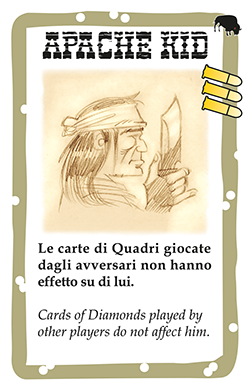
\includegraphics[width=\cardSize\linewidth]{postavy/03_apache_kid.png}
 \caption[Apache Kid]{Nemajú na neho vplyv kárové (diamantové) karty. Pri kartách (Rag time, Springfield etc.) kde sa spolu s danou kartou odhadzuje ďaľšia bez efektu nemôže byť ani jedna károva. Môžte proti nemu použiť károve: Vedle!, Zbraň (modrá) a Bang! počas duelu,}
  \label{fig:bang}
\end{minipage}
\hfill
\begin{minipage}[t]{\minipageSize}\centering
  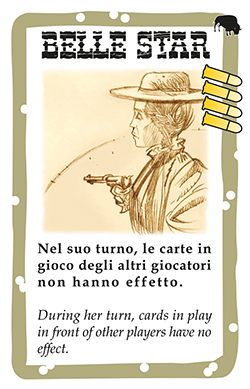
\includegraphics[width=\cardSize\linewidth]{postavy/03_belle_star.png}
  \caption[Belle Star]{Počas jej ťahu nemajú karty (modré a zelené) vyložené pred ostatnými hráčmi efekt.}
  \label{fig:vedle}
\end{minipage}
\hfill
\begin{minipage}[t]{\minipageSize}\centering
  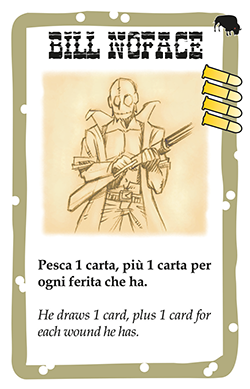
\includegraphics[width=\cardSize\linewidth]{postavy/03_bill_noface.png}
  \caption[Bill Noface]{Vo fáze 1 potiahne 1 kartu, plus 1 kartu za každý stratený život. Tento základ sa potom upravuje ďalšími efektmi, ktoré menia počet ťahaných kariet vo fáze 1, napr. Smädom alebo Príchodom vlaku.}
  \label{fig:duel}
\end{minipage}
\hfill
\begin{minipage}[t]{\minipageSize}\centering
  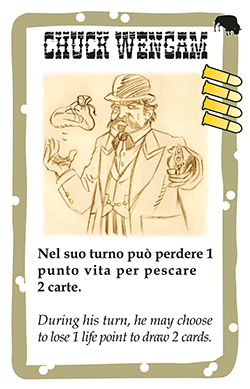
\includegraphics[width=\cardSize\linewidth]{postavy/03_chuck_wengam.png}
\caption[Chuck Wengam]{Vo svojom ťahu môže stratiť 1 život a za to potiahnúť 2 karty. Túto schopnosť môže použiť viackrát za ťah, ale nemôže sa ňou sám vyradiť. Ak je v hre ako duch bez životov, schopnosť použiť nemôže, pokiaľ si najprv neobnoví aspoň 1 život.}
  \label{fig:panico}
\end{minipage}
\end{figure}

\begin{figure}[!h]
\begin{minipage}[t]{\minipageSize}\centering
  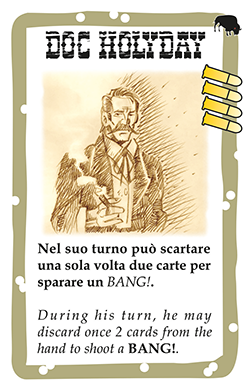
\includegraphics[width=\cardSize\linewidth]{postavy/03_doc_holyday.png}
 \caption[Doc Holyday]{Raz za svoj ťah môže odhodiť 2 karty a tým vyvolať efekt Bang! na dostrel. Tento efekt sa nepočíta do limitu Bang!. Ak ho chce použiť proti Apache Kidovi, aspoň jedna z odhodených kariet musí byť iná než kárová.}
  \label{fig:bang}
\end{minipage}
\hfill
\begin{minipage}[t]{\minipageSize}\centering
  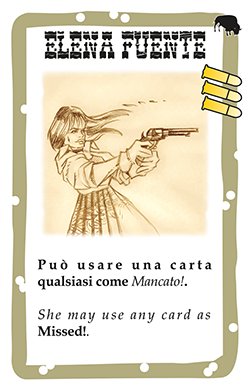
\includegraphics[width=\cardSize\linewidth]{postavy/03_elena_fuente.png}
  \caption[Elena Fuente]{Môže zahrať ľubovoľnú kartu z ruky ako efekt Vedle!.}
  \label{fig:vedle}
\end{minipage}
\hfill
\begin{minipage}[t]{\minipageSize}\centering
  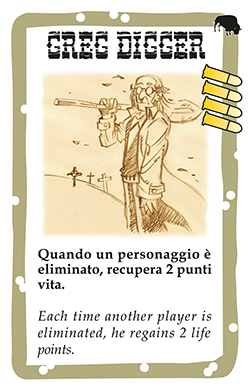
\includegraphics[width=\cardSize\linewidth]{postavy/03_greg_digger.png}
  \caption[Greg Digger]{Vždy keď je iná postava vyradená z hry, doplní si 2 životy v rámci limitu. Platí to aj vtedy, keď z hry odchádza duch pri karte Město duchů z High Noon.}
  \label{fig:duel}
\end{minipage}
\hfill
\begin{minipage}[t]{\minipageSize}\centering
  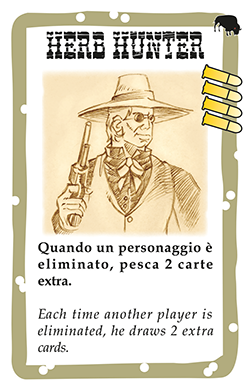
\includegraphics[width=\cardSize\linewidth]{postavy/03_herb_hunter.png}
\caption[Herb Hunter]{Vždy keď je iná postava vyradená z hry, potiahne si 2 karty. V prípade, že zabije banditu, potiahne si spolu 5 kariet. Platí to aj vtedy, keď z hry odchádza duch pri karte Město duchů z High Noon.}
  \label{fig:panico}
\end{minipage}
\end{figure}

\begin{figure}[!h]
\begin{minipage}[t]{\minipageSize}\centering
  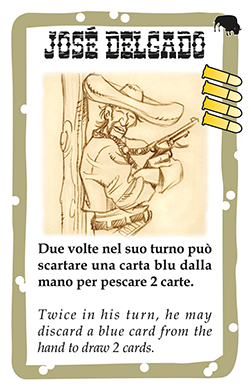
\includegraphics[width=\cardSize\linewidth]{postavy/03_jose_delgado.png}
 \caption[Jose Delgado]{Vo svojom ťahu môže odhodiť z ruky modrú kartu a ťahať 2 karty z balíka. Túto schopnosť môže použiť len 2x za kolo.}
  \label{fig:bang}
\end{minipage}
\hfill
\begin{minipage}[t]{\minipageSize}\centering
  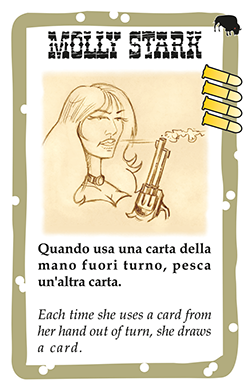
\includegraphics[width=\cardSize\linewidth]{postavy/03_molly_stark.png}
  \caption[Molly Stark]{Vždy, keď dobrovoľne zahrá kartu mimo svojho ťahu, potiahne si 1 kartu z balíčka. Platí to napríklad pri kartách alebo efektoch Vedle!, Pivo či Indiáni. Pri Dueli si potiahne toľko kariet, koľko odhodila kariet Bang!, ale až po jeho skončení. Schopnosť sa nevzťahuje na Cat Balou ani Panico!.}
  \label{fig:vedle}
\end{minipage}
\hfill
\begin{minipage}[t]{\minipageSize}\centering
  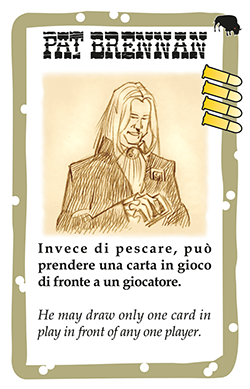
\includegraphics[width=\cardSize\linewidth]{postavy/03_pat_brennan.png}
  \caption[Pat Brennan]{Môže preskočiť fázu 1 a zobrať si jednu kartu (modrá, zelená) zo stola. }
  \label{fig:duel}
\end{minipage}
\hfill
\begin{minipage}[t]{\minipageSize}\centering
  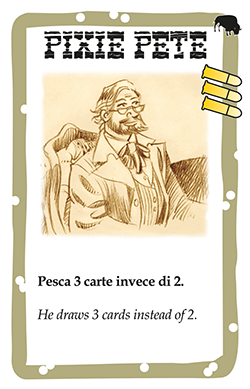
\includegraphics[width=\cardSize\linewidth]{postavy/03_pixie_pete.png}
\caption[Pixie Pete]{Vo fáze 1 si potiahne 3 karty namiesto 2. Ak vstúpi do hry ako duch pri Měste duchů, tiež si vo fáze 1 potiahne 3 karty.}
  \label{fig:panico}
\end{minipage}
\end{figure}

\begin{figure}[!h]
\begin{minipage}[t]{\minipageSize}\centering
  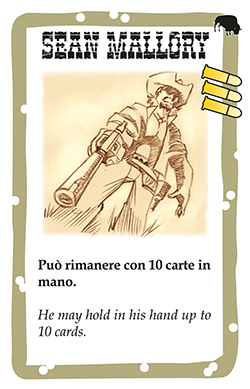
\includegraphics[width=\cardSize\linewidth]{postavy/03_sean_mallory.png}
 \caption[Sean Mallory]{Vo svojom ťahu vo fáze 3 môže mať na ruke až 10 kariet bez toho aby ich musel odhadzovať.}
  \label{fig:bang}
\end{minipage}
\hfill
\begin{minipage}[t]{\minipageSize}\centering
  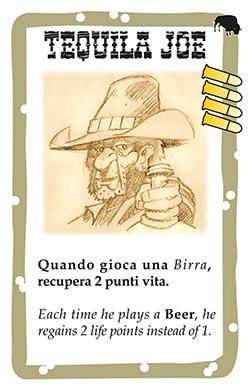
\includegraphics[width=\cardSize\linewidth]{postavy/03_tequila_joe.png}
  \caption[Tequila Joe]{Vždy keď zahrá kartu Pivo, pridáva si 2 životy namiesto 1. Platí to iba pre konkrétnu kartu Pivo, nie pre iné efekty Pivo. Ak je na poslednom živote a má na ruke iba 1 kartu Pivo, zachráni sa ňou pred bežným zranením na 2 životy; proti Dynamitu však môže na prežitie potrebovať viac kariet Pivo podľa celkovej straty životov.}
  \label{fig:vedle}
\end{minipage}
\hfill
\begin{minipage}[t]{\minipageSize}\centering
  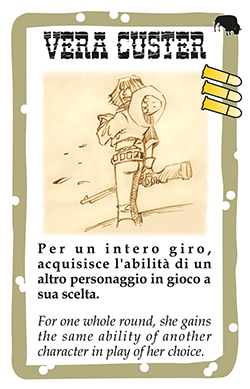
\includegraphics[width=\cardSize\linewidth]{postavy/03_vera_custer.png}
  \caption[Vera Custer]{Na začiatku svojho ťahu pred fázou 1 si vyberie inú postavu (stále v hre) ktorej schopnosti skopíruje. Tieto schopnosti sú platné až do začiatku jej daľšieho kola. Ak Vera Custer skopíruje schopnosť Gary Lootera tak sa v zbieraní odhodených kariet striedajú. Začína ten kto je bližšie po ľavici hráča ktorý kartu odhodil. Tento princíp platí aj pre Vulture Sam schopnosť etc.}
  \label{fig:duel}
\end{minipage}
\hfill
\begin{minipage}[t]{\minipageSize}\centering
  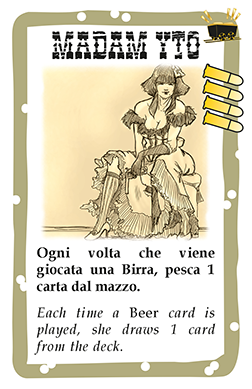
\includegraphics[width=\cardSize\linewidth]{postavy/04_madame_yto.png}
\caption[Madam Yto]{Vždy, keď niekto zahrá kartu Pivo, potiahne si 1 kartu z balíčka. Platí to aj pre vlastnú kartu Pivo. Nezáleží na tom, či sa karta Pivo zahrala na liečenie alebo na získanie zlatého nugetu. Schopnosť sa nevzťahuje na iné karty s podobným efektom, napr. Whisky alebo Bottle.}
  \label{fig:panico}
\end{minipage}
\end{figure}

\begin{figure}[!h]
\begin{minipage}[t]{\minipageSize}\centering
  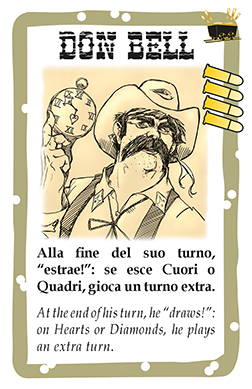
\includegraphics[width=\cardSize\linewidth]{postavy/04_don_bell.png}
 \caption[Don Bell]{Na konci svojho ťahu ťahá kartu. Ak je červená, odohrá ešte jeden celý ťah od fázy 1. Takto získaný extra ťah už nemôže znovu spustiť jeho vlastnú schopnosť.}
  \label{fig:bang}
\end{minipage}
\hfill
\begin{minipage}[t]{\minipageSize}\centering
  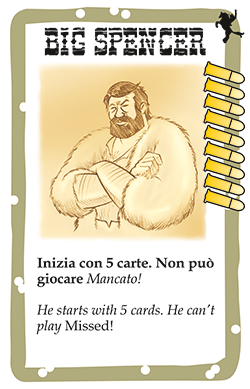
\includegraphics[width=\cardSize\linewidth]{postavy/06_bigspencer.png}
  \caption[Big Spencer]{Začína s 5 kartami. Nemôže hrať kartu Vedle!, ale môže používať iné karty a schopnosti, ktoré vytvárajú efekt Vedle!, napr. Bibliu alebo Barel.}
  \label{fig:vedle}
\end{minipage}
\hfill
\begin{minipage}[t]{\minipageSize}\centering
  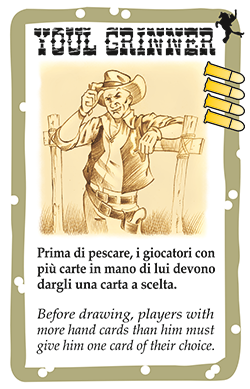
\includegraphics[width=\cardSize\linewidth]{postavy/06_youlgrinner.png}
  \caption[Youl Grinner]{Pred fázou 1, a teda až po všetkých ťahoch na Dynamit, Väzenie a podobné karty, mu každý hráč, ktorý má viac kariet na ruke než Youl, musí dať 1 kartu podľa svojho výberu. Ak takých hráčov je viac, kartu mu dá každý z nich.}
  \label{fig:duel}
\end{minipage}
\hfill
\begin{minipage}[t]{\minipageSize}\centering
  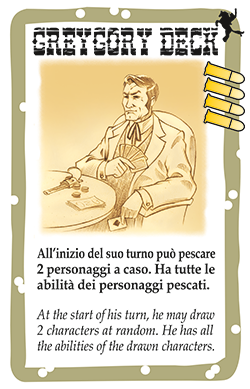
\includegraphics[width=\cardSize\linewidth]{postavy/06_greygorydeck.png}
\caption[Greygory Deck]{Na začiatku hry a potom na začiatku každého svojho ťahu si môže náhodne zobrať dve postavy zo základnej hry. Tieto postavy nesmú byť v hre. Má všetky schopnosti oboch postáv. Ak si ich chce vymeniť, musí vymeniť obe naraz, nie iba jednu; pôvodné postavy sa zamiešajú späť medzi ostatné a až potom sa ťahajú nové. Ak sú dve skopírované schopnosti v priamom rozpore, vyberie si, ktorú použije, inak platia obe.}
  \label{fig:panico}
\end{minipage}
\end{figure}


\begin{figure}[!h]
\begin{minipage}[t]{\minipageSize}\centering
  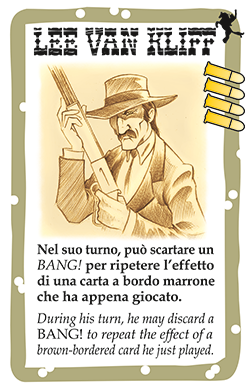
\includegraphics[width=\cardSize\linewidth]{postavy/06_leevankliff.png}
 \caption[Lee Van Kliff]{Počas svojho ťahu môže odhodiť kartu Bang!, aby zopakoval efekt hnedej karty, ktorú práve zahral. Takto môže zopakovať aj ďalšiu kartu Bang!, ak ňou bola pôvodná hnedá karta. Každú konkrétnu kartu však môže touto schopnosťou zopakovať iba raz. Pri posudzovaní interakcií, napr. s Apache Kidom, je rozhodujúca kopírovaná karta, nie odhodená karta Bang!. Ak kopíruje Rvačku a podobné karty, nemusí odhadzovať ďalšiu kartu navyše.}
  \label{fig:bang}
\end{minipage}
\hfill
\begin{minipage}[t]{\minipageSize}\centering
  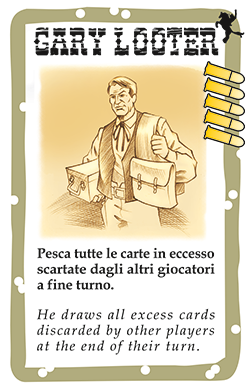
\includegraphics[width=\cardSize\linewidth]{postavy/06_garylooter.png}
  \caption[Gary Looter]{Berie si všetky prebytočné karty z odhadzovacieho balíčka, ktoré hráči vyhodia fo fáze 3.}
  \label{fig:vedle}
\end{minipage}
\hfill
\begin{minipage}[t]{\minipageSize}\centering
  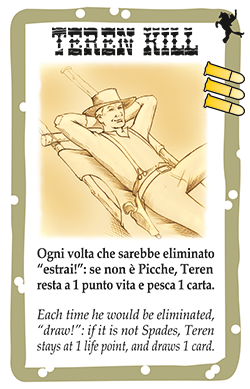
\includegraphics[width=\cardSize\linewidth]{postavy/06_terenkill.png}
  \caption[Teren Kill]{Pokiaľ by mal byť vyradený z hry, môže sa rozhodnúť, či sa zachráni bežným spôsobom, napr. kartou Pivo, alebo použije svoju schopnosť a ťahá kartu z balíčka. Pokiaľ to nie sú piky, ostane na 1 živote a potiahne si 1 kartu. Platí to vo všetkých prípadoch, bez ohľadu na to, koľko životov mu má byť odobraných. Po neúspešnom ťahaní už nemôže hrať kartu Pivo ani na neho nemožno zahrať kartu Obetavý skok.}
  \label{fig:duel}
\end{minipage}
\hfill
\begin{minipage}[t]{\minipageSize}\centering
  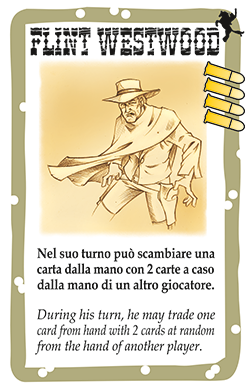
\includegraphics[width=\cardSize\linewidth]{postavy/06_flintwestwood.png}
\caption[Flint Westwood]{Počas svojho ťahu si môže raz vymeniť jednu kartu zo svojej ruky za jednu kartu z ruky ľubovoľného hráča podľa vlastného výberu. Ak má cieľový hráč na ruke iba jednu kartu, Flint získa práve túto kartu.}
  \label{fig:panico}
\end{minipage}
\end{figure}

\begin{figure}[!h]
\begin{minipage}[t]{\minipageSize}\centering
  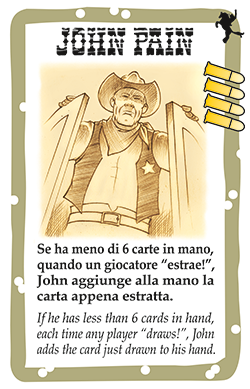
\includegraphics[width=\cardSize\linewidth]{postavy/06_johnpain.png}
 \caption[John Pain]{Vždy, keď nejaký hráč ťahá kartu na zistenie efektu, John Pain si môže vziať otočenú kartu do ruky, ak má menej ako 6 kariet. Platí to aj pri dvoch kartách ťahaných schopnosťou Lucky Duke; ak má v tom momente už 5 kariet, získa iba prvú z nich. Nevzťahuje sa to na automatické ťahy, napr. pri Helene Zontero. Kartu získanú týmto spôsobom nemožno použiť okamžite na ten istý práve vyhodnocovaný efekt.}
  \label{fig:bang}
\end{minipage}
\hfill
\begin{minipage}[t]{\minipageSize}\centering
  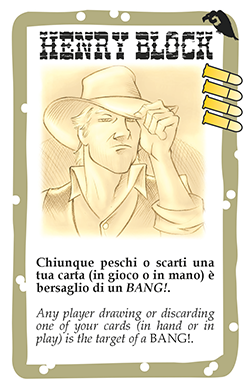
\includegraphics[width=\cardSize\linewidth]{postavy/07_henryblock.png}
 \caption[Henry Block]{Hráč, ktorý odoberie alebo odhodí kartu z Henryho ruky, alebo z kariet ležiacich pred ním, je cieľom efektu Bang!. Tento automatický výstrel sa vždy vyhodnotí skôr, než sa dokončí pôvodné dobratie alebo odhodenie karty. Platí to aj pri kartách namierených na všetkých hráčov ako napríklad "Risa". Henry Block nespúšta efekt karty Odmena. \\
 Neplatí pri: Flint Westwood, Youl Grinner, El Gringo.\\
 Platí pri: Jesse Jonesovi a Pat Brennanovi.\\ Schopnosť nespustí ani výstrel z Brokovnice.  }
  \label{fig:bang}
\end{minipage}
\hfill
\begin{minipage}[t]{\minipageSize}\centering
  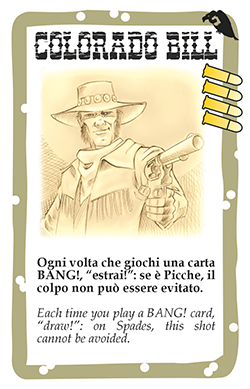
\includegraphics[width=\cardSize\linewidth]{postavy/07_coloradobill.png}
  \caption[Colorado Bill]{Vždy, keď niekto zahrá kartu Vedle! proti jeho karte Bang!, Colorado Bill môže ťahať vrchnú kartu balíčka. Ak je to pika, efekt tejto karty Vedle! sa ignoruje. Platí to len pri konkrétnych kartách Bang! a Vedle!, nie pri iných efektoch Bang! alebo Vedle!. Ak sa jeho schopnosť úspešne vyhodnotí, proti tejto karte Bang! už nemožno použiť Barel ani schopnosť postavy Jourdonnais.}
  \label{fig:vedle}
\end{minipage}
\hfill
\begin{minipage}[t]{\minipageSize}\centering
  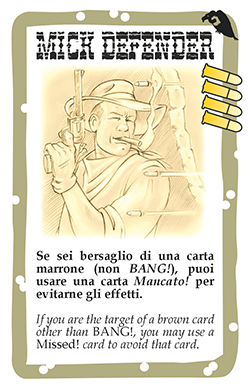
\includegraphics[width=\cardSize\linewidth]{postavy/07_mickdefender.png}
  \caption[Mick Defender]{Keď sa stane cieľom karty alebo efektu, môže zahrať kartu Vedle! a vyhnúť sa jej účinku na seba. Platí to aj proti kartám, ktoré zasahujú viacerých hráčov, napr. Indiáni alebo Guľomet, ale zruší ich iba vo vzťahu k Mickovi. Keď sú v hre už len dvaja hráči, môže túto schopnosť používať normálne.}
  \label{fig:duel}
\end{minipage}





\end{figure}

\begin{figure}[!h]
\begin{minipage}[t]{\minipageSize}\centering
  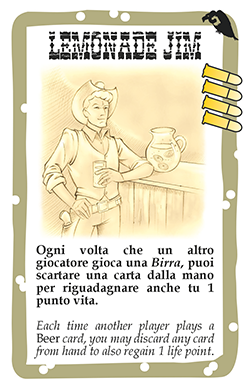
\includegraphics[width=\cardSize\linewidth]{postavy/07_lemonadejim.png}
\caption[Limonádový Jim]{Vždy, keď niektorý hráč zahrá kartu Pivo, Jim môže odhodiť ľubovoľnú kartu a získať efekt Pivo.}
  \label{fig:panico}
\end{minipage}
\hfill
\begin{minipage}[t]{\minipageSize}\centering
  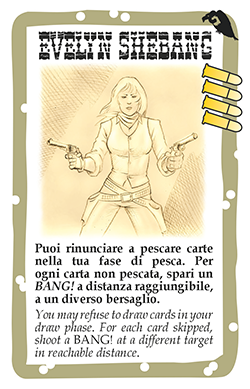
\includegraphics[width=\cardSize\linewidth]{postavy/07_evelynshebang.png}
 \caption[Evelyn Shebang]{Vo fáze 1 sa ešte pred ťahaním musí rozhodnúť, či si potiahne o 0, 1 alebo 2 karty menej. Za každú takto nepotiahnutú kartu automaticky vyvolá 1 efekt Bang! na vzdialenosť 1. Vzdialenosť upravujú karty vyložené pred hráčmi.}
  \label{fig:bang}
\end{minipage}
\hfill
\begin{minipage}[t]{\minipageSize}\centering
  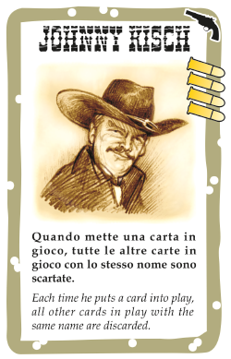
\includegraphics[width=\cardSize\linewidth]{postavy/bonus-johnny-kisch.png}
  \caption[Johnny Kisch]{Vždy, keď vyloží kartu do hry, všetky ostatné karty v hre s rovnakým názvom sa odhodia. Platí to pre karty, ktoré sa vykladajú do hry, teda najmä modré a zelené karty vrátane Väzenia.}
  \label{fig:vedle}
\end{minipage}
\hfill
\begin{minipage}[t]{\minipageSize}\centering
  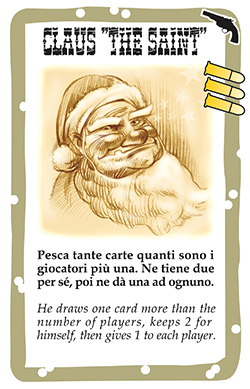
\includegraphics[width=\cardSize\linewidth]{postavy/bonus-ClausTheSaint.png}
  \caption[Claus The Saint]{Počas svojej fáze 1 vyberie o jednu kartu naviac ako je hráčov, dve si nechá a ostatné rozdá podľa seba.}
  \label{fig:duel}
\end{minipage}
\hfill
\begin{minipage}[t]{\minipageSize}\centering
  \fbox{\parbox[c][0.18\textheight][c]{0.72\linewidth}{\centering Bonus postava\\bez obrázka}}
  \caption[Emiliano]{Keď je jeho karta Bang! zrušená kartou Vedle!, vezme si túto kartu Vedle! do ruky. Keď sa on sám vyhne karte Bang!, vezme si túto kartu Bang! do ruky.}
  \label{fig:emiliano}
\end{minipage}
\hfill
\begin{minipage}[t]{\minipageSize}\centering
  \fbox{\parbox[c][0.18\textheight][c]{0.72\linewidth}{\centering Bonus postava\\bez obrázka}}
  \caption[Annie Versary]{Môže zahrať ľubovoľnú kartu z ruky ako kartu Bang!.}
  \label{fig:annieversary}
\end{minipage}
\end{figure}

\begin{figure}[!h]

\begin{minipage}[t]{\minipageSize}\centering
  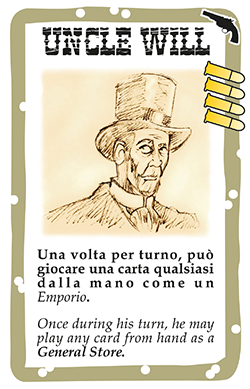
\includegraphics[width=\cardSize\linewidth]{postavy/bonus-UncleWill.png}
\caption[Uncle Will]{Raz za svoj ťah môže zahrať hociakú kartu z ruky ako Hokynářství.}
  \label{fig:panico}
\end{minipage}
   \begin{minipage}[t]{\minipageSize}\centering
      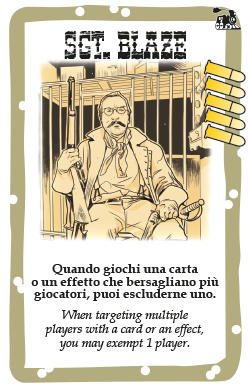
\includegraphics[width=\cardSize\linewidth]{postavy/25_SgtBlaze.png}
      \caption[Sgt. Blaze]{Keď zahráte kartu alebo vyvoláte efekt, ktorý zasahuje viacerých hráčov, môžete jedného hráča z tohto efektu vyňať. Pri Hokynářství otočíte o jednu kartu menej. Platí to aj pri efekte lokomotívy na konci trate, ak sa tento efekt spustil počas vášho ťahu.}
    \end{minipage}
    \hfill
    \begin{minipage}[t]{\minipageSize}\centering
      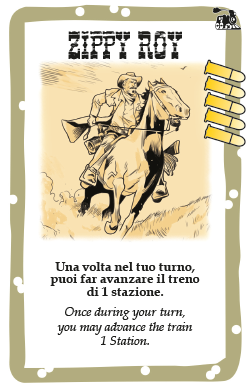
\includegraphics[width=\cardSize\linewidth]{postavy/26_ZippyRoy.png}
      \caption[Zippy Roy]{Raz za ťah môžete posunúť vlak o 1 stanicu dopredu. Touto schopnosťou iba posúvate vlak a nezískavate tým žiadny vagón zadarmo.}
    \end{minipage}
        \hfill
    \begin{minipage}[t]{\minipageSize}\centering
      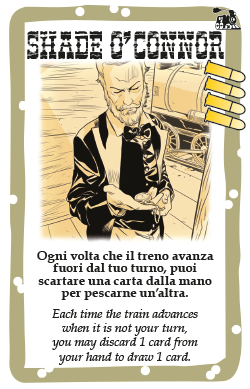
\includegraphics[width=\cardSize\linewidth]{postavy/24_ShadeOConnor.png}
      \caption[Shade O'Connor]{Vždy, keď sa vlak posunie dopredu mimo vášho ťahu, môžete odhodiť 1 kartu a potiahnuť si 1 novú. Ak vlak týmto posunom dôjde na konečnú stanicu, túto výmenu vykonáte ešte pred vyhodnotením efektu lokomotívy.}
    \end{minipage}
\end{figure}

\begin{figure}[!h]
    \begin{minipage}[t]{\minipageSize}\centering
      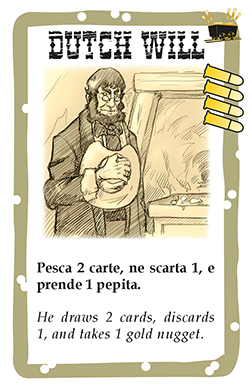
\includegraphics[width=\cardSize\linewidth]{postavy/04_dutch_will.png}
      \caption[Dutch Will]{Počas fázy 1 môže jednu z práve potiahnutých kariet podľa vlastného výberu odhodiť a získať za to 1 valún zlata.}
    \end{minipage}
    \hfill
    \begin{minipage}[t]{\minipageSize}\centering
      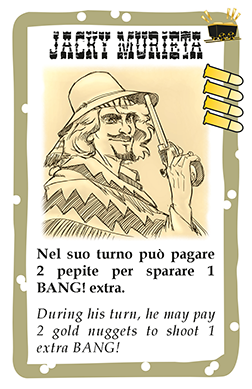
\includegraphics[width=\cardSize\linewidth]{postavy/04_jacky_murieta.png}
      \caption[Jacky Murieta]{Môže za 2 valúny zlata vyvolať efekt Bang! na hráča na dostrel. Tento efekt sa nepočíta do limitu Bang! a schopnosť môže použiť viackrát za ťah, ak má dosť zlata. Nehrá pritom žiadnu kartu Bang!.}
    \end{minipage}
    \hfill
    \begin{minipage}[t]{\minipageSize}\centering
      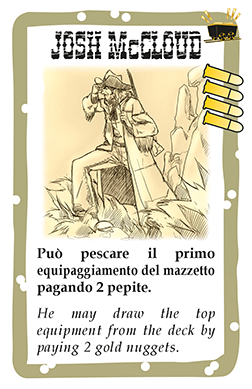
\includegraphics[width=\cardSize\linewidth]{postavy/04_josh_mccloud.png}
      \caption[Josh McCloud]{Počas svojho ťahu môže za cenu 2 valúnov zlata potiahnuť kartu z balíčka vybavenia. Ak potiahne čiernu kartu vybavenia, ktorú už má vyloženú, musí ju odhodiť.}
    \end{minipage}
    \hfill
    \begin{minipage}[t]{\minipageSize}\centering
      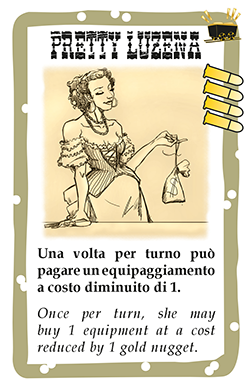
\includegraphics[width=\cardSize\linewidth]{postavy/04_pretty_luzena.png}
      \caption[Pretty Luzena]{Počas každého svojho ťahu môže kúpiť 1 kartu vybavenia so zľavou 1 valúna zlata. Ak dané vybavenie stojí 1 valún, získa ho zadarmo. Ostatné vybavenie v tom istom ťahu už platí v plnej cene.}
    \end{minipage}
\end{figure}

\begin{figure}[!h]
    \begin{minipage}[t]{\minipageSize}\centering
      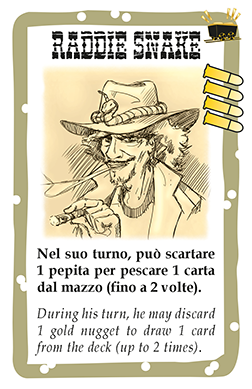
\includegraphics[width=\cardSize\linewidth]{postavy/04_raddie_snake.png}
      \caption[Raddie Snake]{Dvakrát za ťah môže odhodiť 1 valún zlata a potiahnuť si 1 kartu z balíčka.}
    \end{minipage}
    \hfill
    \begin{minipage}[t]{\minipageSize}\centering
      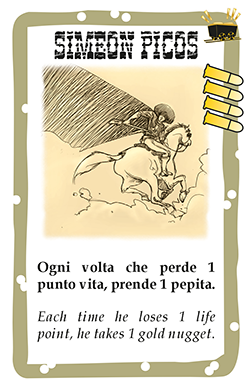
\includegraphics[width=\cardSize\linewidth]{postavy/04_simeon_picos.png}
      \caption[Simeon Picos]{Vždy, keď stratí 1 život, vezme si 1 valún zlata zo spoločnej zásoby. Valún berie vždy zo zásoby, nie od hráča alebo zdroja, ktorý mu život odobral.}
    \end{minipage}
    \hfill
    \begin{minipage}[t]{\minipageSize}\centering
      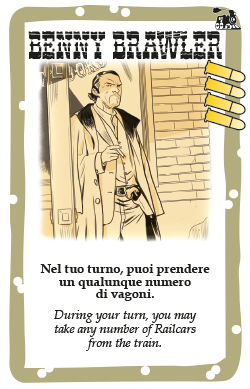
\includegraphics[width=\cardSize\linewidth]{postavy/19_BennyBrawler.png}
      \caption[Benny Brawler]{Môže za ťah získať neobmedzený počet vagónov. Každý ďalší vagón však stále musí normálne zaplatiť; zadarmo môže získať najviac ten prvý, na ktorý by mal inak nárok.}
    \end{minipage}
    \hfill
    \begin{minipage}[t]{\minipageSize}\centering
      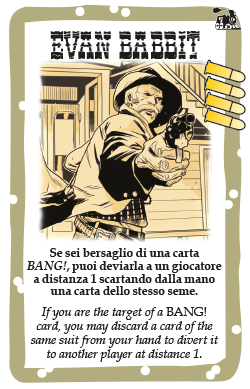
\includegraphics[width=\cardSize\linewidth]{postavy/20_EvanBabbit.png}
      \caption[Evan Babbit]{Ak ste cieľom karty Bang!, môžete odhodiť kartu s rovnakým symbolom a odkloniť tým efekt Bang! na iného hráča vo vzdialenosti 1 od Evana. Túto vzdialenosť neovplyvňujú karty vyložené na stole. Nový cieľ nesmie byť pôvodný útočiaci hráč a pri dvoch zostávajúcich hráčoch schopnosť nemožno použiť. Odklonený efekt Bang! sa stále považuje za efekt pôvodného útočiaceho hráča, takže všetky odmeny a postihy sa vyhodnocujú voči nemu.}
    \end{minipage}
\end{figure}

\begin{figure}[!h]
    \begin{minipage}[t]{\minipageSize}\centering
      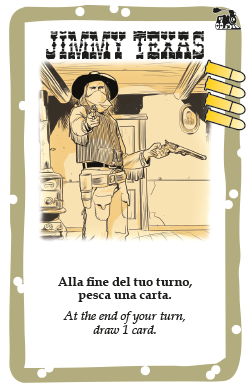
\includegraphics[width=\cardSize\linewidth]{postavy/21_JimmyTexas.png}
      \caption[Jimmy Texas]{Na konci svojho ťahu si potiahne 1 kartu z balíčka. Platí to aj v prípade, že sa v danom kole nedostal z Väzenia. Táto karta sa ťahá až po odhadzovaní prebytočných kariet, takže ju už v tom istom ťahu nemožno zahrať.}
    \end{minipage}
    \hfill
    \begin{minipage}[t]{\minipageSize}\centering
      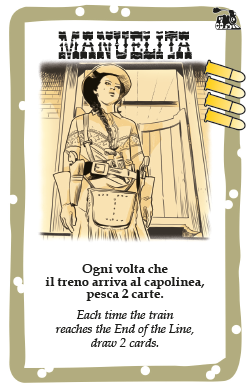
\includegraphics[width=\cardSize\linewidth]{postavy/22_Manuelita.png}
      \caption[Manuelita]{Vždy keď vlak dôjde na konečnú stanicu, potiahnite si dve karty z balíka. Schopnosť sa aplikuje pred efektom lokomotívy. }
    \end{minipage}
    \hfill
    \begin{minipage}[t]{\minipageSize}\centering
      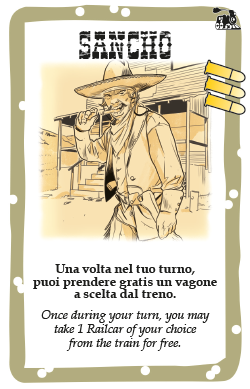
\includegraphics[width=\cardSize\linewidth]{postavy/23_Sancho.png}
      \caption[Sancho]{Raz za ťah môžete získať 1 ľubovoľný vagón zadarmo. Predtým môžete podľa potreby posunúť vlak. Takto získaný vagón sa počíta do bežného limitu vagónov za ťah.}
    \end{minipage}
    \hfill
    \begin{minipage}[t]{\minipageSize}\centering

    \end{minipage}
   
    

\end{figure}
